%%%%%%%%%%%%%%%%%%%%%%%%%%%%%%%%%%%%%%%%%%  不使用 authblk 包制作标题  %%%%%%%%%%%%%%%%%%%%%%%%%%%%%%%%%%%%%%%%%%%%%%
%-------------------------------PPT Title-------------------------------------
\title{06-赝势理论与总能量求和}
%-----------------------------------------------------------------------------

%----------------------------Author & Date------------------------------------
%\author[\textrm{Jun\_Jiang}]{姜\;\;骏\inst{}} %[]{} (optional, use only with lots of authors)
%% - Give the names in the same order as the appear in the paper.
%% - Use the \inst{?} command only if the authors have different
%%   affiliation.
%\institute[BCC]{\inst{}%
\institute[Gain~Strong]{\inst{}%
%\vskip -20pt 北京市计算中心}
\vskip -20pt {\large 格致斯创~科技}}
\date[\today] % (optional, should be abbreviation of conference name)
{%	{\fontsize{6.2pt}{4.2pt}\selectfont{\textcolor{blue}{E-mail:~}\url{jiangjun@bcc.ac.cn}}}
\vskip 45 pt {\fontsize{8.2pt}{6.2pt}\selectfont{%清华大学\;\;物理系% 报告地点
	\vskip 5 pt \textrm{2023.02.11}}}
}

%% - Either use conference name or its abbreviation
%% - Not really information to the audience, more for people (including
%%   yourself) who are reading the slides onlin%%   yourself) who are reading the slides onlin%%   yourself) who are reading the slides onlineee
%%%%%%%%%%%%%%%%%%%%%%%%%%%%%%%%%%%%%%%%%%%%%%%%%%%%%%%%%%%%%%%%%%%%%%%%%%%%%%%%%%%%%%%%%%%%%%%%%%%%%%%%%%%%%%%%%%%%%

\subject{}
% This is only inserted into the PDF information catalog. Can be left
% out.
%\maketitle
\frame
{
%	\frametitle{\fontsize{9.5pt}{5.2pt}\selectfont{\textcolor{orange}{“高通量并发式材料计算算法与软件”年度检查}}}
\titlepage
}
%-----------------------------------------------------------------------------

%------------------------------------------------------------------------------列出全文 outline ---------------------------------------------------------------------------------
%\section*{}
%\frame[allowframebreaks]
%{
%  \frametitle{Outline}
%%  \frametitle{\textcolor{mycolor}{\secname}}
%  \tableofcontents%[current,currentsection,currentsubsection]
%}
%%在每个section之前列出全部Outline
%%类似的在每个subsection之前列出全部Outline是\AtBeginSubsection[]
%\AtBeginSection[]
%{
%  \frame<handout:0>%[allowframebreaks]
%  {
%    \frametitle{Outline}
%%全部Outline中,本部分加亮
%    \tableofcontents[current,currentsection]
%  }
%}

%-----------------------------------------------PPT main Body------------------------------------------------------------------------------------
\small
\subsection{基态总能量表达式}
\frame
{
	\frametitle{晶体总能量的一般表示\footnote{本部分参阅文献\cite{JPC-SSP12-4409_1979,Xie_Lu,Elect_Stru}}}
采用赝势方法计算的晶体总能量$E_T$由晶格中的电子能量$E_{e-e}$与离子实排斥能$E_{N-N}$之和:
	\begin{displaymath}
		E_T=E_{e-e}+E_{N-N}=\textcolor{blue}{T[\rho]+E_{ext}+E_{\mathrm{Coul}}}+E_{\mathrm{XC}}+E_{N-N}
	\end{displaymath}
根据\textrm{Kohn-Sham}方程,其中动能泛函用单电子能量表示为
\begin{displaymath}
	T[{\rho}]=\sum_in_i\langle\psi_i|\varepsilon_i-V_{\mathrm{KS}}|\psi_i\rangle
\end{displaymath}
$n_i$是$\psi_i$上的电子占据数,$\varepsilon_i$是其能量本征值,因此有
\begin{displaymath}
	\hspace*{-12.0pt}	E_T=i\textcolor{blue}{\sum_in_i\varepsilon_i-\dfrac12\int\int\mathrm{d}\vec r\mathrm{d}\vec r\dfrac{\rho(\vec r)\rho(\vec r^{\prime})}{|\vec r-\vec r^{\prime}|}}+\int\mathrm{d}\vec r\rho(\vec r)[\epsilon_{\mathrm{XC}}(\vec r)-V_{\mathrm{XC}}(\vec r)]+E_{N-N}
\end{displaymath}
}

\frame
{
	\frametitle{晶体总能量倒空间的表示}
周期体系的总能量表达式在动量空间($\vec K$空间)计算更方便
\begin{displaymath}
	\hspace*{-15.0pt}	E_T=\textcolor{red}{\sum_in_i\varepsilon_i}-\dfrac{\Omega}2\sum_{\textcolor{red}{\vec k\neq 0}}\rho^{\ast}(\vec k)V_{\mathrm{Coul}}(\vec k)+\Omega\sum_{\vec k}\rho^{\ast}(\vec k)[\epsilon_{\mathrm{XC}}(\vec k)-V_{\mathrm{XC}}(\vec k)]+\textcolor{red}{E_{N-N}}
\end{displaymath}
其中$V_{\mathrm{Coul}}(\vec k)$、$\epsilon_{\mathrm{XC}}(\vec k)$与$\rho^{\ast}(\vec k)$分别是\textrm{Coulomb}相互作用、单个电子的交换-相关能、交换-相关势和电子密度的\textrm{Fourier}分量。

由\textrm{Poisson}方程
\begin{displaymath}
	\nabla^2V_{\mathrm{Coul}}(\vec r)=-4\pi\rho(\vec r)
\end{displaymath}
的\textrm{Fourier}展开有
\begin{displaymath}
	V_{\mathrm{Coul}}(\vec k)=\dfrac{4\pi\rho^{\ast}(\vec k)}{|\vec k|^2}
\end{displaymath}
交换-相关势和交换-相关能的计算一般先在实空间计算$\epsilon_{\mathrm{XC}}(\vec r)$和$V_{\mathrm{XC}}(\vec r)$后,再通过\textrm{Fourier}变换到动量空间,得到$\epsilon_{\mathrm{XC}}(\vec k)$和$V_{\mathrm{XC}}(\vec k)$
}

\frame
{
	\frametitle{晶体离子相互作用的计算}
	离子间\textrm{Coulomb}相互作用能之和
	\begin{displaymath}
		E_{N-N}=\dfrac12\sum_{\vec R,s}\sideset{}{^{\prime}}\sum_{\vec R^{\prime},\vec s^{\prime}}\dfrac{Z_sZ_{s^{\prime}}}{|\vec R+\vec r_s-\vec R^{\prime}-\vec r_s^{\prime}|}
	\end{displaymath}
	这里$Z_s$是离子实的电荷数,$\vec R$表示晶格点的位矢,$\vec r_s$代表元胞内原子的相对位矢。

	\textcolor{red}{\textbf{注意}}:~$E_{N-N}$求和有无穷多项,\textcolor{red}{是发散的};~$V_{\mathrm{Coul}}(\vec k=0)$\textcolor{red}{是发散的}
	
	$V_{ext}$在不存在其他外场时,一般只考虑离子-电子的\textrm{Coulomb}相互作用,
	\begin{displaymath}
%		\begin{aligned}
			V_{ext}(\vec r)=\sum_{\vec R,s}\dfrac{-Z_s}{|\vec r-\vec R-\vec r_s|}\equiv\sum_{\vec R,s}v_{ext}^s(\vec r-\vec R-\vec r_s)
%		\end{aligned}
	\end{displaymath}
	$V_{ext}$的\textrm{Fourier}分量在$\vec k=0$\textcolor{red}{也是发散的}
}

\frame
{
	\frametitle{晶体总能量计算的奇点排除}
这三项单独都是发散的,但因为整个体系出于电中性,所以这些发散项相互抵消,是一个常数。因此求解\textrm{Kohn-Sham}方程时,先将$V_{\mathrm{Coul}}(\vec k=0)$和$V_{ext}(\vec k=0)$同时置为零,这相当于\textcolor{red}{将势能作一平移,或者说重新定义势能零点,而在总能量计算中补偿这一平移。}
\begin{figure}[h!]
	\begin{center}
		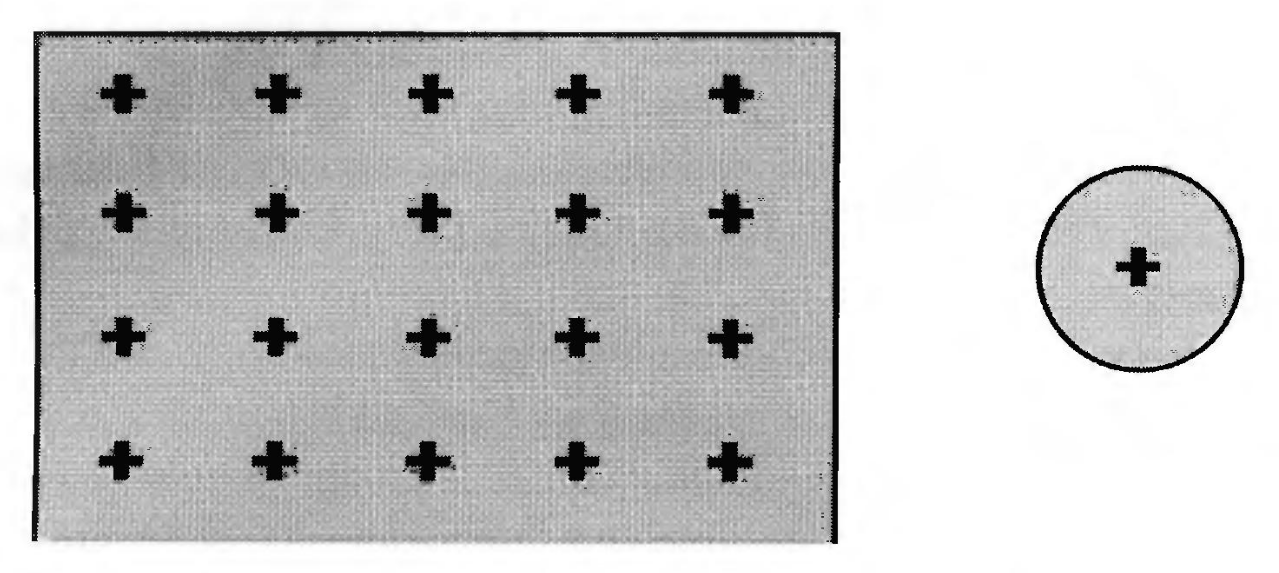
\includegraphics[height=0.65in,width=1.50in,viewport=0 0 1250 565,clip]{Figures/Ewald_method-3.png}
	\end{center}
	\caption{\fontsize{5.5pt}{2.2pt}\selectfont{\textrm{A lattice of point charge in a uniform compensating background as considered in the Ewald calculation.}}}
	\label{fig:Ewald-method-3}
\end{figure}
	发散项之和为:
	\begin{displaymath}
		\begin{aligned}
			\lim_{\vec k\rightarrow0}\Omega&\bigg[\dfrac12V_{\mathrm{Coul}}(\vec k)+\sum_sv_{ext}^s(\vec k)\bigg]\rho^{\ast}(\vec k)+\dfrac12\sum_{\vec R,s}\sideset{}{^{\prime}}\sum_{\vec R^{\prime},\vec s^{\prime}}\dfrac{Z_sZ_{s^{\prime}}}{|\vec R+\vec r_s-\vec R^{\prime}-\vec r_s^{\prime}|}\\
			=&\sum_s\alpha_s\sum_sZ_s+E_{\mathrm{Ewald}}
		\end{aligned}
	\end{displaymath}
}

\frame
{
	\frametitle{发散项的处理}
	对于形如$Z_s/r$的外场,其\textrm{Fourier}分量在$\vec k=0$附近展开
	\begin{displaymath}
		v_{ext}^s(\vec k)=-\dfrac{4\pi Z_s}{\Omega|\vec k|^2}+\alpha_s+O(\vec k); 
	\end{displaymath}
	展开$\rho^{\ast}(\vec k)$,有
	\begin{displaymath}
		\lim_{\vec k\rightarrow 0}\rho^{\ast}(\vec k)=\dfrac{\sum_sZ_s}{\Omega}+\beta|\vec k|^2+O(\vec k)
	\end{displaymath}
去掉高次项,有
\fontsize{8.5pt}{5.2pt}\selectfont{
\begin{displaymath}
	\begin{aligned}
		\lim_{\vec k\rightarrow 0}&\bigg[\boxed{\textcolor{blue}{\dfrac{\Omega}2\dfrac{4\pi[\rho^{\ast}(\vec k)]^2}{|\vec k|^2}}}+\boxed{\Omega}\bigg(\boxed{\textcolor{blue}{-\dfrac{4\pi\sum_sZ_s}{\Omega|\vec k|^2}}}+\sum_s\alpha_s\bigg)\boxed{\rho^{\ast}(\vec k)}+\boxed{\textcolor{red}{\dfrac12\dfrac{4\pi(\sum_sZ_s)^2}{\Omega|\vec k|^2}}}\bigg]\\
		&+\boxed{\dfrac12\sum_{\vec R,s}\sideset{}{^{\prime}}\sum_{\vec R^{\prime},\vec s^{\prime}}\dfrac{Z_sZ_{s^{\prime}}}{|\vec R+\vec r_s-\vec R^{\prime}-\vec r_{s^{\prime}}|}-\lim_{\vec k\rightarrow0}\textcolor{red}{\dfrac12\dfrac{4\pi(\sum_sZ_s)^2}{\Omega|\vec k|^2}}}\\
		=&\sum_s\alpha_s\sum_sZ_s+\textcolor{magenta}{E_{\mathrm{Ewald}}}
	\end{aligned}
\end{displaymath}}
}

\frame
{
	\frametitle{离子间相互作用的\textrm{Ewald}求和}
\begin{figure}[h!]
\centering
\vspace*{-0.20in}
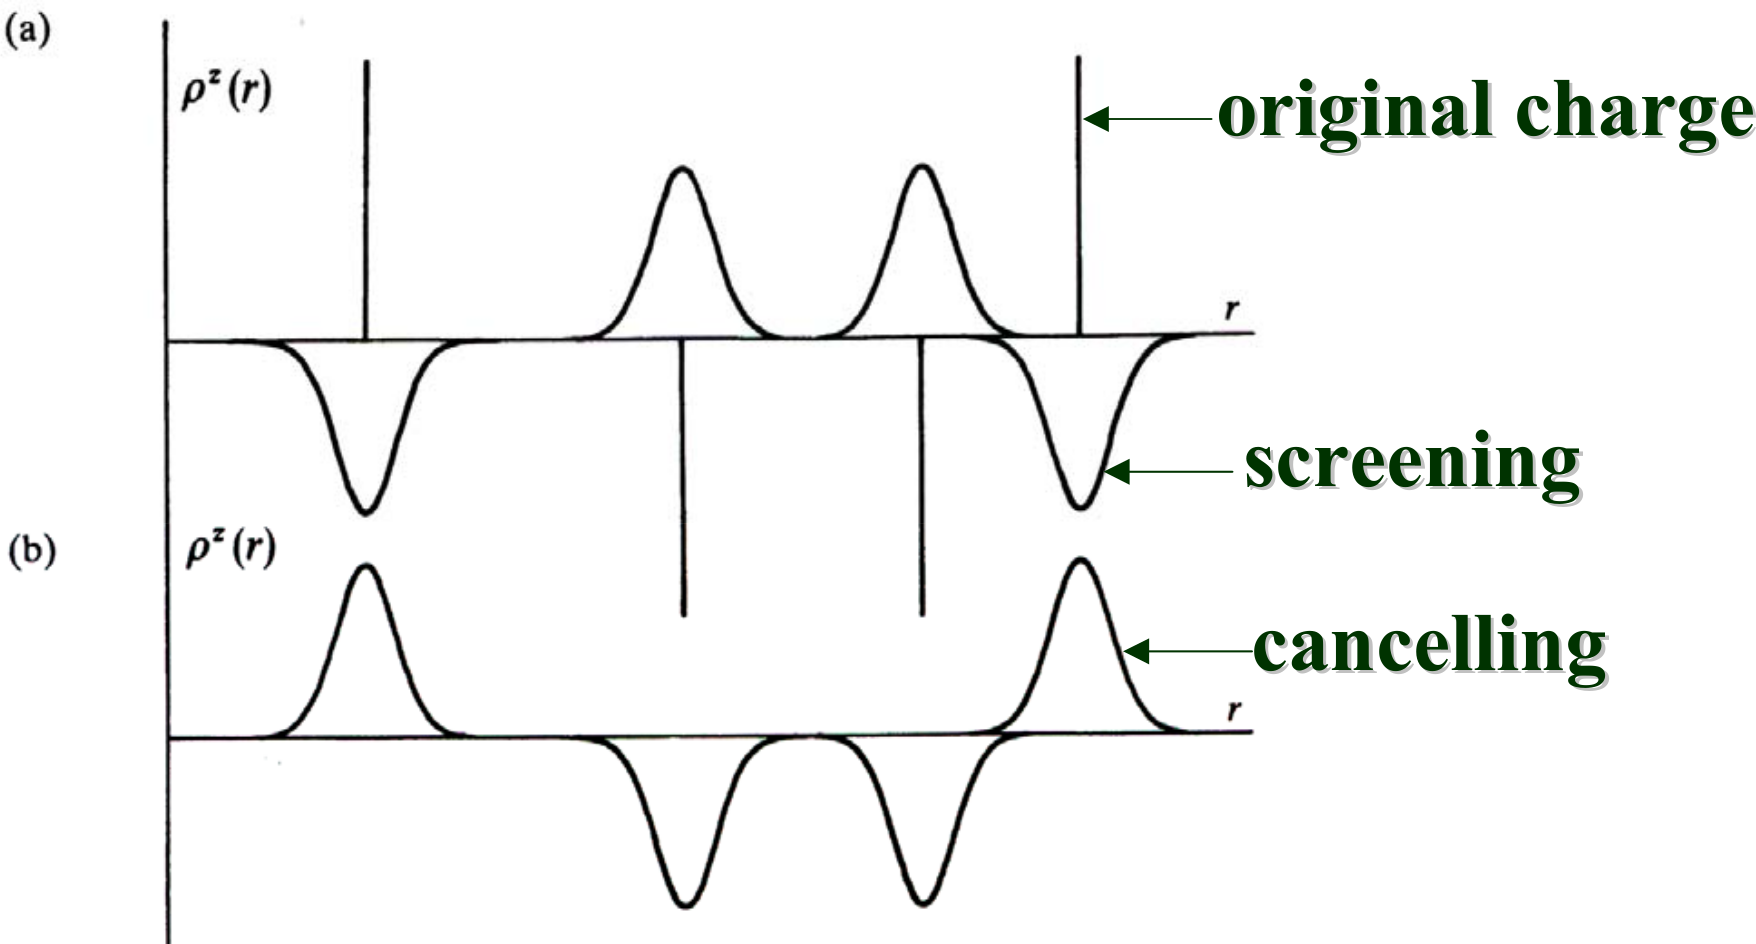
\includegraphics[height=2.3in,width=4.12in,viewport=0 0 1800 955,clip]{Figures/Ewald_method-2.png}
\caption{\fontsize{5.5pt}{2.2pt}\selectfont{\textrm{Each charge be screened by a Gaussian charge distribution of opposite sign and equal magnitude: $\rho_i(r)=\dfrac{Z_i\eta^3}{\pi^{3/2}}\mathrm{e}^{-\eta^2r^2}$.}}}%(与文献\cite{EPJB33-47_2003}图1对比)
\label{Ewald_method-2}
\end{figure}
}

\frame
{
	\frametitle{离子间相互作用的\textrm{Ewald}求和}
\begin{figure}[h!]
\centering
%\vspace*{-0.20in}
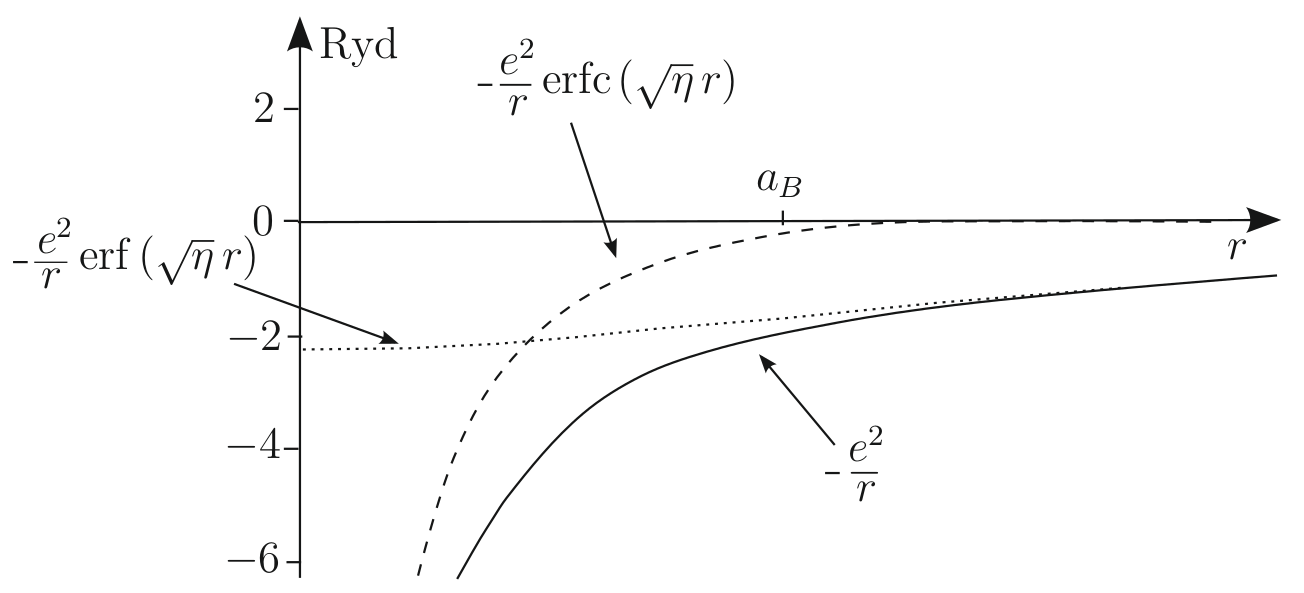
\includegraphics[height=1.8in,width=4.12in,viewport=0 0 1100 455,clip]{Figures/Ewald_method.png}
\caption{\fontsize{5.5pt}{2.2pt}\selectfont{\textrm{Decomposition of the potential $-e^2/r$ (singular at the origin and of long-range nature) into a contribution $-(e^2/r)\mathrm{erf}(\sqrt{\eta}r)$(regular at the origin of long-range) and a contribution $-(e^2/r)\mathrm{erfc}(\sqrt{\eta}r)$ (singular at the origin and of short-range nature). Here $\sqrt{\eta}=1 (\mathrm{Bohr radius unit})$ is chosen.}}}%(与文献\cite{EPJB33-47_2003}图1对比)
\label{Error_Function}
\end{figure}
}

\frame
{
	\frametitle{离子间相互作用的\textrm{Ewald}求和}
	\begin{displaymath}
		\begin{aligned}
			E_{\textrm{Ewald}}=&\dfrac12\sum_{\vec R,s}\sideset{}{^{\prime}}\sum_{\vec R^{\prime},\vec s^{\prime}}\dfrac{Z_sZ_{s^{\prime}}}{|\vec R+\vec r_s-\vec R^{\prime}-\vec r_{s^{\prime}}|}-\lim_{\vec k\rightarrow0}\dfrac12\times\dfrac{4\pi(\sum_sZ_s)^2}{\Omega|\vec k|^2}\\
			=&\dfrac12\sum_{\vec R,s}\sideset{}{^{\prime}}\sum_{\vec R^{\prime},\vec s^{\prime}}\dfrac{Z_sZ_{s^{\prime}}}{|\vec R+\vec r_s-\vec R^{\prime}-\vec r_{s^{\prime}}|}-\dfrac1{2\Omega}\sum_{s,s^{\prime}}\int\mathrm{d}\vec r\dfrac{Z_sZ_{s^{\prime}}}r\\
			=&\sum_{s,s^{\prime}}Z_sZ_{s^{\prime}}\bigg\{\dfrac{2\pi}{\Omega}\sum_{\vec k\neq 0}\cos[\vec k\cdot(\vec r_s-\vec r_{s^{\prime}})]\dfrac{\mathrm{e}^{-|\vec k|^2/4\eta^2}}{|\vec k|^2}\\
			&-\dfrac{\pi}{2\eta^2\Omega}+\dfrac12\sum_{\vec R}\dfrac{\mathrm{erf}(\eta x)}x\bigg|_{\vec R+\vec r_s-\vec r_s^{\prime}\neq0}-\dfrac{\eta}{\sqrt{\pi}}\delta_{s,s^{\prime}}\bigg\}
		\end{aligned}
	\end{displaymath}
	$\mathrm{erf}(x)$是误差函数,$\eta$原则上是任意参数。$\alpha_s$由$v_{ext}^s(\vec r)$确定:
	\begin{displaymath}
		\alpha_s=\lim_{\vec k\rightarrow0}\bigg[v_{ext}^s(\vec k)+\dfrac{4\pi Z_s}{\Omega|\vec k|^2}\bigg]=\dfrac1{\Omega}\int\mathrm{d}\vec r\bigg[v_{ext}^s(\vec r)+\dfrac{Z_s}r\bigg]
	\end{displaymath}
}

\frame
{
	\frametitle{总能量表达式}
\fontsize{6.5pt}{4.2pt}\selectfont{
由此得到的总能量表达式是
\begin{displaymath}
	\begin{aligned}
		E_T=&\sum_i\varepsilon_i-\dfrac{\Omega}2\sum_{\vec k\neq0}\rho^{\ast}(\vec k)V_{\mathrm{Coul}}(\vec k)\\
		&+\Omega\sum_{\vec k}\rho^{\ast}(\vec k)[\epsilon_{\mathrm{XC}}(\vec k)-V_{\mathrm{XC}}(\vec k)]\\
		&+\sum_s\alpha_s\sum_sZ_s+E_{\mathrm{Ewald}}
	\end{aligned}
\end{displaymath}
}
\begin{figure}[h!]
\centering
\vspace*{-0.18in}
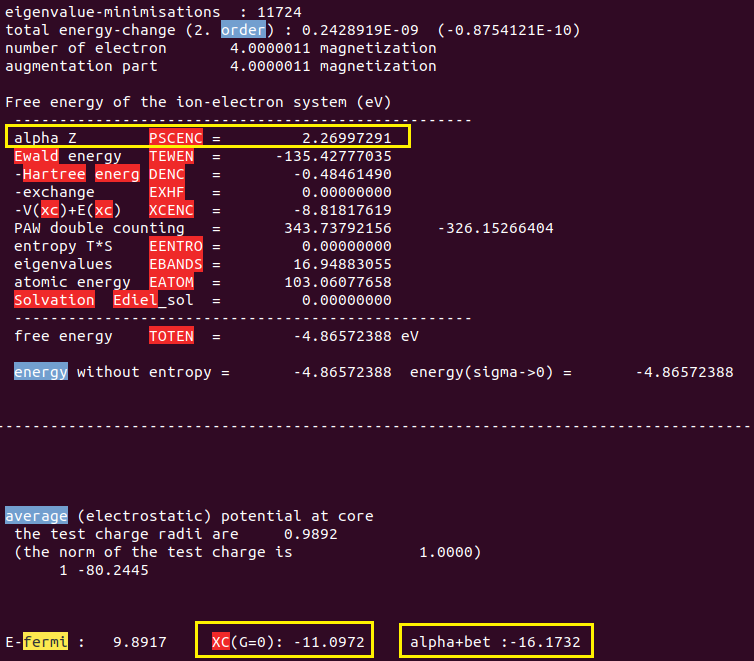
\includegraphics[height=1.85in,width=2.2in,viewport=0 0 600 495,clip]{Figures/VASP_Total_ENE.png}
\caption{\tiny \textrm{The Total-E calculated by VASP.}}%(与文献\cite{EPJB33-47_2003}图1对比)
\label{TOTEN_VASP}
\end{figure}
}

\frame
{
	\frametitle{超软赝势的总能量表示}
	根据\textrm{D. Vanderbilt}的超软赝势(\textrm{US-PP})方案
	原子波函数满足$$(T+V_{\mathrm{AE}}-\varepsilon_n)|\psi_n\rangle=0$$
	据此构造原子赝波函数$\phi_n$,在截断半径$r_c^l$处,$\phi_n$与$\psi_n$平滑衔接(不需要模守恒条件)

	类似地,构造局域平滑势$V_{loc}(r)$,在截断半径$r_c^{loc}$处,$V_{loc}(r)$与$V_{\mathrm{AE}}(r)$平滑衔接
	
	构造辅助轨道
	$$|\chi_n\rangle=(\varepsilon_n-T-V_{loc})|\phi_n\rangle$$
	由此构造内积矩阵,矩阵元$$B_{nm}=\langle\phi_n|\chi_m\rangle$$
	并有$$|\beta_n\rangle=\sum_m(B^{-1})_{mn}|\chi_m\rangle$$
	这里$\beta_n$是局域函数,并与$\phi_n$垂直
}

\frame
{
	\frametitle{\textrm{US-PP}的总能量表示}
	定义\textcolor{orange}{缀加函数}$$Q_{nm}(\vec r)=\psi_n^{\ast}(\vec r)\psi_m(\vec r)-\phi_n^{\ast}(\vec r)\phi_m(\vec r)$$
	\textcolor{blue}{可赝化的补偿电荷}$$q_{nm}=\langle\psi_n|\psi_m\rangle_R-\langle\phi_n|\phi_m\rangle_R$$
	由此可以导出$\phi_n$满足久期方程
	\begin{displaymath}
		\begin{aligned}
			&\left(T+V_{loc}+\sum_{nm}D_{nm}|\beta_n\rangle\langle\beta_m|\right)|\phi_n\rangle\\
			=&\varepsilon_n\left(1+\sum_{nm}q_{nm}|\beta_n\rangle\langle\beta_m|\right)|\phi_n\rangle
		\end{aligned}
	\end{displaymath}
	其中$$D_{nm}=B_{nm}+\varepsilon_nq_{nm}$$
}

\frame
{
	\frametitle{\textrm{US-PP}的总能量表示}
	在超软赝势方法中,包含$N_v$个价电子体系的总能量\upcite{PRB47-10142_1993}
	\begin{displaymath}
		\begin{aligned}
			E_{\mathrm{tot}}[\{\phi_i\},\{\vec R_I\}]=&\sum_i\langle\phi_i|-\frac12\nabla^2+V_{\mathrm{NL}}|\phi_i\rangle\\
			&+\frac12\iint\mathrm{d}\vec r\mathrm{d}\vec r\,^{\prime}\dfrac{n(\vec r)n(\vec r\,^{\prime})}{|\vec r-\vec r\,^{\prime}|}\\
			&+\int\mathrm{d}\vec r V_{loc}^{\mathrm{ion}}(\vec r)n(\vec r)+E_{\mathrm{XC}}[n]\\
			&+U(\{\vec R_I\})
		\end{aligned}
	\end{displaymath}
	这里$\phi$是体系波函数,$n(\vec r)$是电子密度,$E_{\mathrm{XC}}$是交换-相关能,$U(\{\vec R_I\})$是离子-离子相互作用能
}

\frame
{
	\frametitle{\textrm{US-PP}的总能量表示}
	电荷密度$$n(\vec r)=\sum_i\big[|\phi_i(\vec r)|^2+\sum_{nm,I}Q_{nm}^I(\vec r)\langle\phi_i|\beta_n^I\rangle\langle\beta_m^I|\phi_i\rangle\big]$$
	局域势$$V_{loc}^{\mathrm{ion}}(\vec r)=\sum_IV_{loc}^{\mathrm{ion}}(\vec r-\vec R_I)$$
	$V_{loc}^{\mathrm{ion}}$由$V_{loc}$去屏蔽后得到$$V_{loc}^{\mathrm{ion}}(r)=V_{loc}(r)-\int\mathrm{d}\vec r\,^{\prime}\dfrac{n(\vec r\,^{\prime})}{|\vec r-\vec r\,^{\prime}|}-\mu_{\mathrm{XC}}(r)$$
	非局域部分$$V_{\mathrm{NL}}=\sum_{nm,I}D_{nm}^{(0)}|\beta_n^I\rangle\langle\beta_m^I|$$
	这里$$D_{nm}^{(0)}=D_{nm}-\int\mathrm{d}\vec r\,^{\prime}V_{loc}(\vec r\,^{\prime})n(\vec r\,^{\prime})$$
}

\frame
{
	\frametitle{超软赝势总能量计算}
	去除价电子屏蔽效应的贡献后,可得最终超软赝势的总能量表达式
	\begin{displaymath}
		\begin{aligned}
			E_{\mathrm{total}}=&\sum_j^{\mathrm{occ}}\langle\phi_{lmj}|\bigg[-\dfrac12\nabla^2+V_{\mathrm{local}}^{\mathrm{ion}}+\sum_{s,s^{\prime}}\mathbf{D}_{s,s^{\prime}}^{\mathrm{ion}}|\beta_s\rangle\langle\beta_{s^{\prime}}|\bigg]|\phi_{lmj}\rangle\\
			&+E_{H}[n_v]+E_{N-N}+E_{XC}[n_v]
		\end{aligned}
	\end{displaymath}
	{\fontsize{7.2pt}{5.2pt}\selectfont{其中$n_v(r)=\sum\limits_j^{\mathrm{occ}}\phi_{lmj}^{\ast}(r)\phi_{lmj}(r)+\sum\limits_{s,s^{\prime}}\sum\limits_j^{\mathrm{occ}}\langle\phi_{lmj}|\beta_{s^{\prime}}\rangle\langle\beta_s|\phi_{lmj}\rangle Q_{s,s^{\prime}}(r)$
	$$V_{\mathrm{local}}^{\mathrm{ion}}=V_{\mathrm{local}}-V_{\mathrm H}-V_{XC}$$
	$$\mathbf{D}_{s,s^{\prime}}^{\mathrm{ion}}=\mathbf{D}_{s,s^{\prime}}-\int\mathrm{d}\vec r\big[V_{\mathrm{H}}(\vec r)+V_{XC}(\vec r)\big]Q_{s,s^{\prime}}(r)$$}}
	由此可得超软赝势的广义本征值方程
	$$\bigg[-\dfrac12\nabla^2+V_{\mathrm{local}}+\tilde V_{NL}^{\mathrm{US}}-\varepsilon_i\bigg(\mathbf{1}+\sum_{s,s^{\prime}}Q_{s,s^{\prime}}|\beta_s\rangle\langle\beta_{s^{\prime}}|\bigg)\bigg]|\phi_{lmi}\rangle=0$$
}

%------------------------------------------------------------------------Reference----------------------------------------------------------------------------------------------
\begin{thebibliography}{99}
\frame[allowframebreaks]
{
\frametitle{主要参考文献}
{\tiny
\bibitem{JPC-SSP12-4409_1979}\textrm{J.~Ihm, A.~Zunger and M.~L.~Cohen. \textit{J.~Phys.~C:~Solid State Phys.} \textbf{12} (1979), 4409}
\bibitem{Xie_Lu}谢希德、陆栋\:主编, {\textit{固体能带理论}}\:复旦大学出版社, 上海, 1998
\bibitem{Elect_Stru}\textrm{Richard.~M.~Martin. \textit{Electronic Structure: Basic Theory and Practical Methods} (Cambridge University Press, Cambridge, England, 2004)}
\bibitem{PRB47-10142_1993}\textrm{K. Laasonen, A. Pasquarello, R. Car, C. Lee and D. Vanderbilt \textit{Phys. Rev.} B, \textbf{47} (1993), 10142}
}
\nocite*{}
}
\end{thebibliography}

%-----------------------------------------------------------------------------
